\chapter{Architecture}
\minitoc

Le domaine de l'imagerie médicale regorge de concepts nouveaux et d'algorithmes complexes. Afin de compenser cette difficulté, nous nous sommes attachés à plusieurs lignes directrices lors de la conception et la réalisation de notre projet, pour que l'application finale soit la plus simple possible.

\begin{itemize}
  \item Garder une architecture la plus simple possible. Chaque classe représente quelque chose de précis.
  \item Ranger les méthodes dans les bonnes classes.
  \item Limiter les attributs des classes afin de limiter les bogues.
  \item Limiter les dépendances externes et au langage. Les langages évoluent vite et il peut être parfois intéressant de pouvoir passer une application sur un autre langage.
\end{itemize}

\section{Diagramme des cas d'utilisation}

Nous avons réalisé un schéma des cas d'utilisations, visible en figure \vref{usecase} afin de synthétiser les besoins de l'utilisateur, pour offrir une vision simplifiée du système. Nous rappellerons brièvement les fonctionnalités par la suite.

\begin{figure}[h]
\begin{center}
    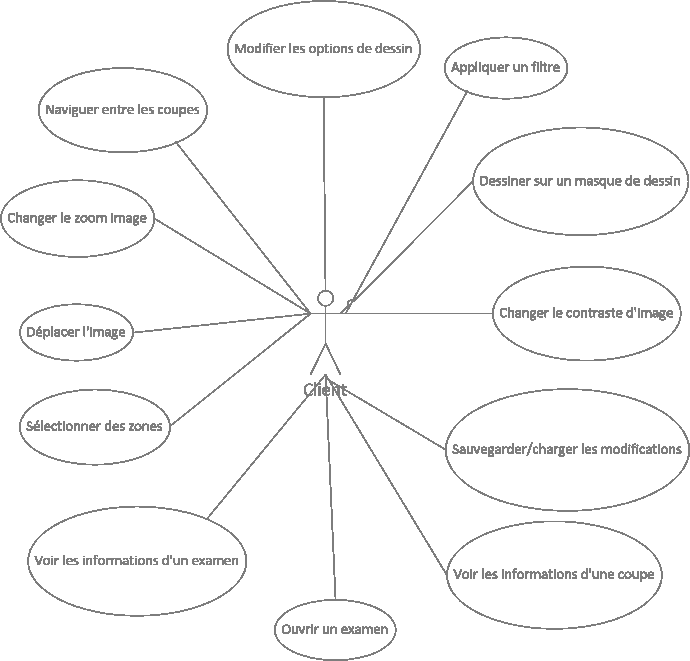
\includegraphics[width=12cm]{diagramme-usecase}
\end{center}
    \caption{Diagramme de cas d'utilisation}
    \label{usecase}                      
\end{figure}

\subsubsection{Ouvrir un examen}

L'utilisateur peut ouvrir un examen stocké sur sa tablette en parcourant l'arborescence de fichiers
et en cliquant sur l'examen choisi.

\subsubsection{Visualiser les informations d'un examen}

Le client peut, n'importe où dans un examen, visualiser les informations associées à cet examen
en cliquant sur un bouton qui déclenchera l'ouverture de la fenêtre d'affichage des informations.
Il pourra y voir des informations sur le patient et sur les conditions d'examen.

\subsubsection{Visualiser les informations d'une coupe}

Le client peut visualiser les informations associées à une coupe
en cliquant sur un bouton qui déclenchera l'ouverture de la fenêtre d'affichage des informations.
Il pourra y voir des informations associées à la coupe affichée à l'écran.

\subsubsection{Naviguer entre les coupes}

Le client peut visualiser les différentes coupes qui composent un examen qu'il a précédemment ouvert
en cliquant sur les boutons associés aux déplacements entre coupes.

\subsubsection{Dessiner des zones sur un masque de dessin}

Le client peut dessiner sur un masque de dessin en superposition avec l'image d'une coupe de l'examen.
Il dispose d'outils de dessin tels que le crayon ou la gomme.

\subsubsection{Modifier les options de dessin}

Le client peut dessiner sur un masque de dessin en variant les effets tels que l'épaisseur du trait
utilisé.

\subsubsection{Modifier le contraste de l'examen}

Le client peut à tout moment changer le contraste (échelle de Hounsfield) des coupes de l'examen ouvert
en utilisant les contrôles associés à cet effet. Il peut modifier la largeur de l'échelle et son centre.
Il peut également choisir un contraste prédéfini parmi une liste de contrastes pour visualiser des éléments
spécifiques tels que les os ou les chairs.

\subsubsection{Se déplacer dans l'image}

Le client peut visualiser différentes portions d'une image en la faisant glisser sur l'écran avec les doigts.

\subsubsection{Changer le niveau de zoom d'une image}

Le client peut modifier le niveau de zoom d'une image en utilisant le contrôle prévu à cet effet.
Il peut augmenter ou diminuer le niveau de zoom.

\subsubsection{Sauvegarder les modifications}

Le client peut enregistrer ses modifications (dessin, contraste par défaut) effectuées sur un examen.

\subsubsection{Restaurer les modifications}

Le client peut charger ses modifications (dessin, contraste par défaut) effectuées auparavant sur un examen.

\subsubsection{Appliquer un filtre}

Le client peut modifier les images d'un examen en appliquant un filtre (tel que le flou gaussien).

\subsubsection{Sélectionner des zones}

Le client peut sélectionner des zones sur une coupe pour appliquer des traitements spécifiquement sur ces
zones.
\section{Les classes}

Les diagrammes de classes de l'architecture du logiciel ont été réalisés à l'aide des logiciel \emph{Architexa} et \emph{UML Lab} intégrés à \emph{Eclipse}. Nous ne parlerons donc que de notre architecture finale, obtenue au fur et à mesure des sprints et refactorings.

Étant donné l'étendue de l'application, nous ne pouvons pas présenter de diagramme UML à la fois complet et lisible dans ce rapport. Commençons donc par obtenir une vue d'ensemble du logiciel à l'aide du diagramme en couches visible en figure \vref{layered-packages}. En bleu, les packages de transformation des données. En vert, les packages utilitaires. En rouge, le cœur de l'application, qui inclut dans des sous-packages le modèle des données, la gestion de cache et les classes d'interface graphique. Les flèches, plus ou moins épaisses, indiquent une dépendance plus ou moins forte d'un package à un autre.
On remarque bien que le package diams constitue le cœur de l'application.
Les packages utilitaires peuvent être changés sans problèmes, car ils ne dépendant pas d'autres packages.
Le package pixelmed constitue une bibliothèque de traitement de fichiers Dicom dont le cœur d'application dépend.
L'enjeu majeur a donc été de rendre l'architecture du cœur d'application la plus flexible possible pour limiter
l'effort requis en cas de changement de bibliothèques.


\begin{figure}[h]
\begin{center}
    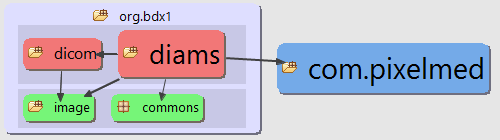
\includegraphics[width=11cm]{diagramme-couche}
\end{center}
    \caption{Diagramme en couches de l'application}
    \label{layered-packages}
\end{figure}

\subsection{Le modèle d'examen}

Voyons maintenant le diagramme des classes du modèle, en figure \vref{classes-model}.
En bleu, les classes utilitaires, en vert le modèle qui représente un examen et les données associées, et en
orange les éléments qui permettent de faire le lien entre le modèle et la bibliothèque d'extraction des images \emph{Pixelmed}.

La classe \verb+DefaultModelFactory+ permet d'interagir depuis l'extérieur avec le modèle d'un examen sans dépendre des autres classes.
La classe \verb+Examen+ est le composant principal qui permet de gérer les autres éléments du modèle.
Un ensemble d'interfaces permet de faciliter des modifications ultérieures sur le modèle.

Notez que la classe orange \verb+LisaImageAdapter+ est le seul élément de dépendance avec la bibliothèque externe \emph{Pixelmed}. Nous avons donc minimisé l'impact que peut créer le passage de \emph{Pixelmed} à un autre outil.


\begin{figure}[h]
\begin{center}
    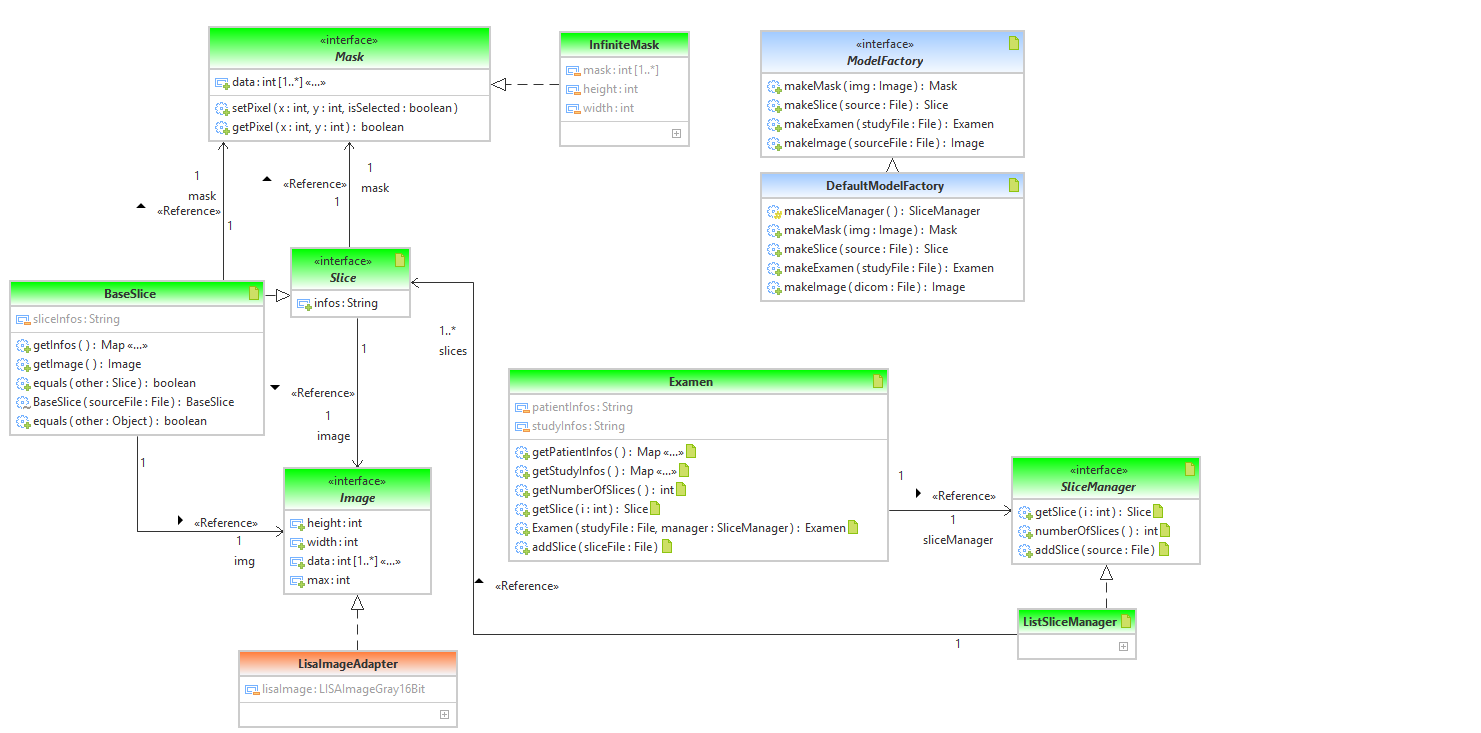
\includegraphics[width=11cm]{diagramme-classes-model}
\end{center}
    \caption{Diagramme de classes du modèle de l'application}
    \label{classes-model}
\end{figure}

\subsection{L'interface graphique}

Nous nous intéressons maintenant au diagramme des classes simplifié de la partie graphique, visible en figure \vref{classes-diams}. En bleu, les classes d'interface graphique. En orange, les classes d'interaction avec les fichiers et en vert la classe d'interaction avec le modèle.

La classe \verb+FileBrowserActivity+ permet, à l'ouverture de l'application, de sélectionner et d'ouvrir un examen parmi une arborescence de fichiers. Les classes \verb+ImageActivity+ et \verb+InfoDisplayActivity+ permettent de visualiser les composants de l'examen choisi et d'interagir avec.
La classe \verb+DicomDirFileHandler+ gère les traitements des fichiers lors de la navigation dans l'arborescence des fichiers.

On note que les dépendances entre l'interface graphique et les données sont limitées à deux classes. Nous avons minimisé l'impact d'un changement de bibliothèque d'interface graphique à ces deux classes.

\begin{figure}[h]
\begin{center}
    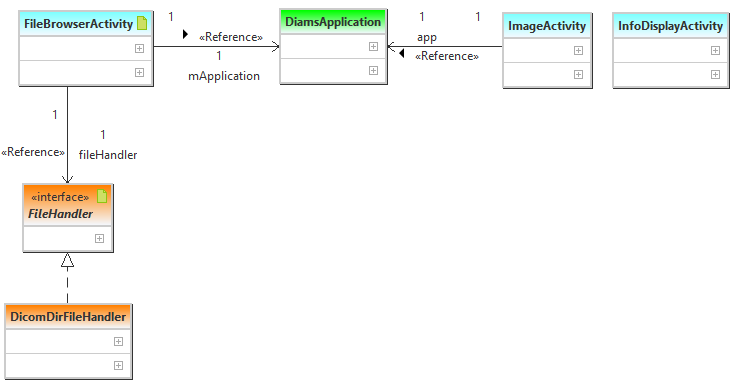
\includegraphics[width=11cm]{diagramme-classes-diams}
\end{center}
    \caption{Diagramme de classes de l'interface graphique de l'application}
    \label{classes-diams}
\end{figure}

\subsection{Le système de cache}

Le développement d'une application mobile entraine des contraintes dues au matériel. La puissance du processeur et la quantité de mémoire vive sont limitées. Notre application devant gérer un grand nombre d'images, nous avons implémenté un système de cache afin de limiter l'occupation mémoire à un instant t, sans pour autant entraver les actions de l'utilisateur par de longs temps de chargement.

Afin que notre couche modèle puisse être réutilisée dans un contexte n'entrainant pas l'utilisation d'un cache, nous avons fait attention à séparer les classes responsables de ce cache des autres classes modèles. Cette problématique nous a tout d'abord conduits à séparer la gestion des coupes de l'Examen proprement dit à travers l'interface \verb+SliceManager+. Nous avons ensuite pu réaliser l'implémentation du cache indépendamment du modèle. La bibliothèque \emph{android} contenant déjà un système de cache, nous avons décidé de l'utiliser pour implémenter \verb+SliceManager+. De cette façon, une seule classe de notre système de cache dépend d'\emph{android}. Enfin, nous utilisons une nouvelle \verb+ModelFactory+ héritant de \verb+DefaultModelFactory+ afin de faire la liaison entre le modèle et le cache.

\begin{figure}[h]
\begin{center}
	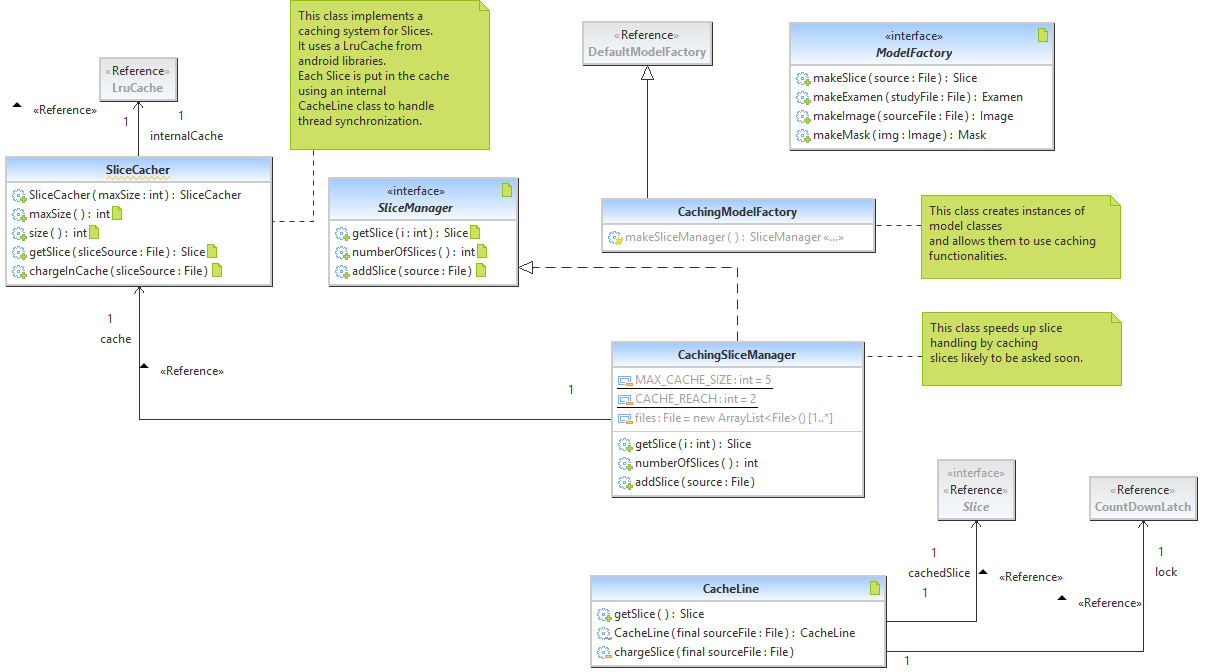
\includegraphics[width=11cm]{diagramme-classes-cache}
\end{center}
	\caption{Diagramme de classes du système de cache}
	\label{classes-cache}
\end{figure}

